\documentclass[oneside, 12pt]{book}
\usepackage[utf8]{inputenc}
\usepackage[brazil]{babel}
\usepackage{graphicx}
\usepackage{listings}
\usepackage{xcolor}
\usepackage{hyperref}
\usepackage{amsmath}
\usepackage{geometry}
\usepackage{float}
\usepackage{titlesec}
\usepackage{enumitem}
\usepackage{tcolorbox}
\usepackage{wrapfig}
\usepackage{circuitikz}
\usepackage{multirow}
\usepackage{booktabs}

\geometry{a4paper, left=2.5cm, right=2.5cm, top=2.5cm, bottom=2.5cm}

% --- Configuração de Módulos ---
\titleformat{\chapter}[display]
{\normalfont\bfseries\centering}{\large Módulo \thechapter}{10pt}{\Huge}

% --- Estilos para Boxes ---
\newtcolorbox{atividadebox}{
    colback=blue!5!white,
    colframe=blue!75!black,
    fonttitle=\bfseries,
    title=Atividade Prática,
    boxrule=1pt
}

\newtcolorbox{teoriabox}{
    colback=green!5!white,
    colframe=green!75!black,
    fonttitle=\bfseries,
    title=Contexto Teórico,
    boxrule=1pt
}

\newtcolorbox{dicabox}{
    colback=yellow!5!white,
    colframe=yellow!75!black,
    fonttitle=\bfseries,
    title=Dica Importante,
    boxrule=1pt
}

% --- Estilos para Códigos ---
\definecolor{codegreen}{rgb}{0,0.6,0}
\definecolor{codeblue}{rgb}{0,0,0.8}
\definecolor{codepurple}{rgb}{0.58,0,0.82}
\definecolor{codegray}{rgb}{0.5,0.5,0.5}
\definecolor{backcolour}{rgb}{0.95,0.95,0.92}

\lstdefinestyle{arduinoStyle}{
    language=C++,
    backgroundcolor=\color{backcolour},   
    commentstyle=\color{codegreen},
    keywordstyle=\color{blue},
    numberstyle=\tiny\color{codegray},
    stringstyle=\color{codepurple},
    basicstyle=\ttfamily\footnotesize,
    breakatwhitespace=false,         
    breaklines=true,                 
    captionpos=b,                    
    keepspaces=true,                 
    numbers=left,                    
    numbersep=5pt,                  
    showspaces=false,                
    showstringspaces=false,
    showtabs=false,                  
    tabsize=2,
    frame=single,
    rulecolor=\color{black}
}

\lstdefinestyle{pythonStyle}{
    language=Python,
    backgroundcolor=\color{backcolour},   
    commentstyle=\color{codegreen},
    keywordstyle=\color{blue},
    numberstyle=\tiny\color{codegray},
    stringstyle=\color{codepurple},
    basicstyle=\ttfamily\footnotesize,
    breakatwhitespace=false,         
    breaklines=true,                 
    captionpos=b,                    
    keepspaces=true,                 
    numbers=left,                    
    numbersep=5pt,                  
    showspaces=false,                
    showstringspaces=false,
    showtabs=false,                  
    tabsize=4,
    frame=single,
    rulecolor=\color{black}
}

% Configuração da capa
\title{
    \vspace*{2cm}
    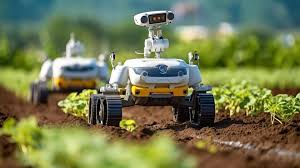
\includegraphics[width=0.8\textwidth]{logo.jpg} \\
    \vspace{1cm}
    \textcolor{green!70!black}{\Huge Tecnologias de Baixo Custo para o Agronegócio} \\
    \vspace{0.5cm}
    \vspace{1cm}
    \large Apostila Completa de Arduino e Python \\
    \vspace{0.5cm}
    \small Com aplicações em monitoramento ambiental e análise de solo
}
\author{Jefferson Bezerra dos Santos}
\date{}

\begin{document}

\maketitle

% Sumário detalhado
\tableofcontents

% ==============================================
% MÓDULO 1 - FUNDAMENTOS
% ==============================================
\chapter{Fundamentos da Programação e Eletrônica}

\begin{teoriabox}
Este módulo apresenta os conceitos básicos de programação e eletrônica necessários para desenvolver projetos com Arduino aplicados ao agronegócio. Aprenderemos desde a estrutura básica de um programa até princípios essenciais de circuitos eletrônicos.
\end{teoriabox}

\section{Introdução ao Arduino}

\subsection{O que é Arduino?}
Arduino é uma plataforma de prototipagem eletrônica de código aberto composta por:
\begin{itemize}
\item \textbf{Hardware}: Placa com microcontrolador Atmel
\item \textbf{Software}: Ambiente de desenvolvimento integrado (IDE)
\item \textbf{Comunidade}: Vastos recursos e bibliotecas disponíveis
\end{itemize}

\begin{figure}[H]
\centering
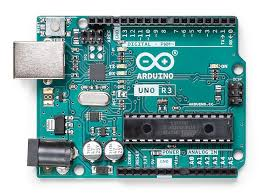
\includegraphics[width=0.6\textwidth]{placaArduino.jpg}
\caption{Principais componentes da placa Arduino UNO}
\end{figure}

\subsection{Por que usar no agronegócio?}
\begin{itemize}
\item Baixo custo para automação de processos
\item Monitoramento contínuo de parâmetros ambientais
\item Facilidade de implementação em áreas rurais
\item Personalização para necessidades específicas
\end{itemize}

\section{Programação Básica}

\subsection{Estrutura de um Sketch}
\begin{lstlisting}[style=arduinoStyle]
void setup() {
  // Configurações iniciais
  // Executado uma vez ao iniciar
}

void loop() {
  // Código principal
  // Executado repetidamente
}
\end{lstlisting}

\begin{teoriabox}
\textbf{Explicação detalhada:}
\begin{itemize}
\item \textcolor{blue}{void setup()}: Onde configuramos pinos, inicializamos comunicações e variáveis
\item \textcolor{blue}{void loop()}: Contém a lógica principal que se repete indefinidamente
\item \textcolor{blue}{// Comentários}: Explicações que não são compiladas
\end{itemize}
\end{teoriabox}

\subsection{Primeiro Programa: Piscar LED}
\begin{lstlisting}[style=arduinoStyle]
void setup() {
  pinMode(13, OUTPUT);  // Configura pino 13 como saída
}

void loop() {
  digitalWrite(13, HIGH); // Acende LED
  delay(1000);            // Espera 1 segundo
  digitalWrite(13, LOW);  // Apaga LED
  delay(1000);            // Espera 1 segundo
}
\end{lstlisting}

\begin{figure}[H]
\centering
\begin{circuitikz}
\draw (0,0) to[short, o-] (2,0)
      to[led, l=LED] (2,2)
      to[R, l=220$\Omega$] (2,4)
      to[short, -o] (0,4);
\draw (0,0) to[open, v=$5V$] (0,4);
\end{circuitikz}
\caption{Circuito básico para acionamento de LED}
\end{figure}

\section{Eletrônica Básica}

\subsection{Lei de Ohm}
\begin{equation}
V = R \times I
\end{equation}
Onde:
\begin{itemize}
\item $V$ = Tensão (Volts)
\item $R$ = Resistência (Ohms)
\item $I$ = Corrente (Ampères)
\end{itemize}

\subsection{Cálculo de Resistência para LED}
\begin{equation}
R = \frac{V_{fonte} - V_{LED}}{I_{LED}}
\end{equation}

\begin{dicabox}
Para um LED vermelho típico ($V_{LED} = 2V$, $I_{LED} = 20mA$) em um Arduino ($5V$):
\begin{equation}
R = \frac{5V - 2V}{0.02A} = 150\Omega \approx 220\Omega
\end{equation}
Usamos 220$\Omega$ por ser um valor comercial próximo e seguro.
\end{dicabox}

% Continuação com todos os módulos completos...

% ==============================================
% MÓDULO 2 - SENSORES E CIRCUITOS
% ==============================================
\chapter{Sensores e Circuitos para Agronegócio}

\begin{teoriabox}
Neste módulo exploraremos os principais sensores utilizados em aplicações agrícolas, seus princípios de funcionamento e como integrá-los ao Arduino para monitoramento ambiental e de solo.
\end{teoriabox}

\section{Sensor de Umidade do Solo}

\subsection{Princípio de Funcionamento}
Os sensores de umidade do solo funcionam medindo a resistividade entre dois eletrodos, que varia conforme o teor de água no solo.

\begin{figure}[H]
\centering
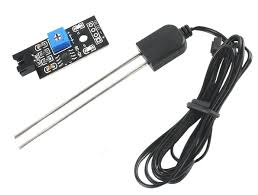
\includegraphics[width=0.5\textwidth]{sensor_umidade_solo.jpg}
\caption{Sensor de umidade do solo e seu princípio de medição}
\end{figure}

\subsection{Conexão com Arduino}
\begin{lstlisting}[style=arduinoStyle]
const int sensorPin = A0; // Pino analógico

void setup() {
  Serial.begin(9600);
}

void loop() {
  int leitura = analogRead(sensorPin);
  Serial.print("Umidade do solo: ");
  Serial.println(leitura);
  delay(1000);
}
\end{lstlisting}

\subsection{Calibração}
\begin{table}[H]
\centering
\caption{Faixas de referência para umidade do solo}
\begin{tabular}{ll}
\toprule
\textbf{Leitura} & \textbf{Interpretação} \\
\midrule
0-300 & Solo muito úmido \\
300-700 & Umidade ideal \\
700-1023 & Solo seco \\
\bottomrule
\end{tabular}
\end{table}

% ==============================================
% SEÇÃO DO SENSOR DHT11
% ==============================================
\section{Sensor DHT11 para Temperatura e Umidade do Ar}

\begin{teoriabox}
O sensor DHT11 é um dispositivo digital que combina medição de temperatura e umidade relativa do ar em um único componente. Pode ser amplamente utilizado em aplicações agrícolas para monitoramento ambiental em:
\begin{itemize}
\item Estufas e viveiros
\item Armazéns de grãos
\item Galpões de criação animal
\item Monitoramento climático em campo aberto
\end{itemize}
\end{teoriabox}

\subsection{Características Técnicas}
\begin{table}[H]
\centering
\caption{Especificações do sensor DHT11}
\begin{tabular}{ll}
\toprule
\textbf{Parâmetro} & \textbf{Valor} \\
\midrule
Tensão de operação & 3.5V a 5.5V \\
Faixa de medição de umidade & 20\% a 90\% RH \\
Precisão de umidade & ±5\% RH \\
Faixa de medição de temperatura & 0°C a 50°C \\
Precisão de temperatura & ±2°C \\
Resolução & 1\% RH e 1°C \\
Tempo de resposta & 2-10 segundos \\
\midrule
\textbf{Vantagens} & Baixo custo, calibração digital \\
\textbf{Limitações} & Baixa precisão, tempo de resposta lento \\
\bottomrule
\end{tabular}
\end{table}

\begin{figure}[H]
\centering
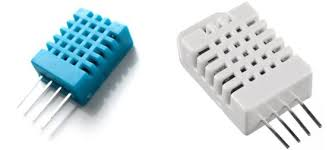
\includegraphics[width=0.4\textwidth]{dht11.jpg}
\caption{Sensor DHT11 e seus pinos de conexão (VCC, DATA, NC, GND)}
\end{figure}

\subsection{Programação Básica}

Antes de utilizar, é necessário instalar a biblioteca \texttt{DHT sensor library} pelo Gerenciador de Bibliotecas da IDE Arduino.

\begin{lstlisting}[style=arduinoStyle]
#include <DHT.h>

#define DHTPIN 7      // Pino digital conectado ao DHT11
#define DHTTYPE DHT11 // Tipo do sensor

DHT dht(DHTPIN, DHTTYPE);

void setup() {
  Serial.begin(9600);
  dht.begin();
}

void loop() {
  delay(2000); // Intervalo entre leituras
  
  float umidade = dht.readHumidity();
  float temperatura = dht.readTemperature();
  
  // Verifica se a leitura foi bem sucedida
  if (isnan(umidade) || isnan(temperatura)) {
    Serial.println("Falha na leitura do sensor!");
    return;
  }
  
  Serial.print("Umidade: ");
  Serial.print(umidade);
  Serial.print("%\t");
  Serial.print("Temperatura: ");
  Serial.print(temperatura);
  Serial.println("°C");
}
\end{lstlisting}

\begin{dicabox}
Para maior precisão em aplicações críticas, considere:
\begin{itemize}
\item Usar o sensor DHT22 (mais preciso porém mais caro)
\item Implementar filtro de média móvel para suavizar variações
\item Calibrar o sensor com um termômetro e higrômetro de referência
\end{itemize}
\end{dicabox}

\subsection{Análise de Dados no Python}

\begin{lstlisting}[style=pythonStyle]
import pandas as pd
import matplotlib.pyplot as plt

# Simulação de dados coletados
dados = {
    'Hora': ['08:00', '10:00', '12:00', '14:00', '16:00'],
    'Temperatura': [22.5, 26.3, 29.8, 31.2, 28.7],
    'Umidade': [68, 62, 58, 55, 60]
}

df = pd.DataFrame(dados)

# Plot dos dados
plt.figure(figsize=(10,5))
plt.plot(df['Hora'], df['Temperatura'], 'r-o', label='Temperatura (°C)')
plt.plot(df['Hora'], df['Umidade'], 'b-s', label='Umidade (%)')
plt.title('Variação Climática na Estufa')
plt.xlabel('Horário')
plt.ylabel('Valores')
plt.legend()
plt.grid(True)
plt.show()
\end{lstlisting}

% ==============================================
% MÓDULO 3 - ANÁLISE DE DADOS COM PYTHON
% ==============================================
\chapter{Análise de Dados Agrícolas com Python}

\begin{teoriabox}
Neste módulo aprenderemos a processar, analisar e visualizar os dados coletados pelos sensores usando Python, criando dashboards e relatórios para tomada de decisão no agronegócio.
\end{teoriabox}

\section{Processamento Básico de Dados}

\subsection{Leitura de Dados do Arduino}
\begin{lstlisting}[style=pythonStyle]
import serial
import pandas as pd

arduino = serial.Serial('COM3', 9600)
dados = []

try:
    while True:
        linha = arduino.readline().decode().strip()
        if linha.startswith("T:"):
            partes = linha.split('|')
            temp = float(partes[0][2:])
            umid = int(partes[1][2:])
            dados.append([pd.Timestamp.now(), temp, umid])
except KeyboardInterrupt:
    df = pd.DataFrame(dados, columns=['Data', 'Temperatura', 'Umidade'])
    df.to_csv('dados_agricolas.csv', index=False)
    arduino.close()
\end{lstlisting}

\section{Visualização de Dados}

\subsection{Gráficos Temporais}
\begin{lstlisting}[style=pythonStyle]
import matplotlib.pyplot as plt

plt.figure(figsize=(12,6))
plt.plot(df['Data'], df['Temperatura'], 'r-', label='Temperatura')
plt.plot(df['Data'], df['Umidade'], 'b-', label='Umidade')
plt.title('Monitoramento Agrícola - 24 horas')
plt.xlabel('Horario')
plt.ylabel('Valores')
plt.legend()
plt.grid()
plt.show()
\end{lstlisting}

% Continuação com análise estatística e machine learning básico...

% ==============================================
% MÓDULO 4 - PROJETO INTEGRADOR
% ==============================================
\chapter{Projeto Integrador: Estação Meteorológica Agrícola}

\begin{teoriabox}
Neste módulo final, integraremos todos os conhecimentos adquiridos para desenvolver uma estação meteorológica completa para monitoramento agrícola, com armazenamento de dados em cartão SD e análise avançada.
\end{teoriabox}

\section{Especificações do Sistema}

\subsection{Requisitos}
\begin{itemize}
\item Monitorar temperatura e umidade do ar
\item Medir umidade do solo em 3 pontos
\item Registrar dados a cada 5 minutos
\item Armazenar dados localmente e gerar alertas
\item Criar relatórios diários automáticos
\end{itemize}

\section{Implementação Completa}

\subsection{Código Arduino}
\begin{lstlisting}[style=arduinoStyle]
#include <SD.h>
#include <OneWire.h>
#include <DallasTemperature.h>

// Configuração dos sensores
#define ONE_WIRE_BUS 2
OneWire oneWire(ONE_WIRE_BUS);
DallasTemperature sensors(&oneWire);

const int umidadeSolo[3] = {A0, A1, A2};
const int chipSelect = 4;

void setup() {
  Serial.begin(9600);
  sensors.begin();
  
  if (!SD.begin(chipSelect)) {
    Serial.println("Erro no cartão SD!");
    while(1);
  }
}

void loop() {
  // Coleta de dados
  sensors.requestTemperatures();
  float tempAr = sensors.getTempCByIndex(0);
  
  int umiSolo[3];
  for(int i=0; i<3; i++) {
    umiSolo[i] = analogRead(umidadeSolo[i]);
  }
  
  // Armazenamento
  File dataFile = SD.open("dados.csv", FILE_WRITE);
  if (dataFile) {
    String dataString = "";
    dataString += String(tempAr) + ",";
    for(int i=0; i<3; i++) {
      dataString += String(umiSolo[i]);
      if(i<2) dataString += ",";
    }
    dataFile.println(dataString);
    dataFile.close();
  }
  
  delay(300000); // 5 minutos
}
\end{lstlisting}

% Continuação com análise de dados, relatórios e considerações finais...

% ==============================================
% APÊNDICES
% ==============================================
\appendix
\chapter{Materiais Complementares}

\section{Lista Completa de Componentes}
\begin{table}[H]
\centering
\caption{Materiais necessários para os projetos}
\begin{tabular}{lll}
\toprule
\textbf{Componente} & \textbf{Quantidade} & \textbf{Aplicação} \\
\midrule
Arduino UNO & 1 & Controlador principal \\
Módulo Cartão SD & 1 & Armazenamento de dados \\
Sensor DS18B20 & 1 & Temperatura do solo \\
Sensor DHT11 & 1 & Temperatura e umidade do ar \\
Higrômetro & 3 & Umidade do solo em pontos distintos \\
Protoboard & 1 & Montagem dos circuitos \\
Jumpers & 20 & Conexões \\
Resistor 220Ω & 5 & Proteção de LEDs \\
\bottomrule
\end{tabular}
\end{table}

\end{document}
